% LaTeX Article Template - customizing header and footer
\documentclass{article}

\newtheorem{thm}{Theorem}

% Set left margin - The default is 1 inch, so the following 
% command sets a 1.25-inch left margin.
\setlength{\oddsidemargin}{0.25in}

% Set width of the text - What is left will be the right margin.
% In this case, right margin is 8.5in - 1.25in - 6in = 1.25in.
\setlength{\textwidth}{6in}

% Set top margin - The default is 1 inch, so the following 
% command sets a 0.75-inch top margin.
\setlength{\topmargin}{-0.25in}

% Set height of the header
\setlength{\headheight}{0.3in}

% Set vertical distance between the header and the text
\setlength{\headsep}{0.2in}

% Set height of the text
\setlength{\textheight}{9in}

% Set vertical distance between the text and the
% bottom of footer
\setlength{\footskip}{0.1in}

% Set the beginning of a LaTeX document
\usepackage{tikz}
\usepackage{multirow}
\usepackage{fullpage}
\usepackage{graphicx}
\usepackage{amsthm}
\usepackage{url}
\usepackage{amssymb}
\usepackage{amssymb}
\usepackage{algpseudocode}
\graphicspath{%
    {converted_graphics/}% inserted by PCTeX
    {/}% inserted by PCTeX
}
%%%%%%%%%%%%%%%%%%%%%%%%%%%%%




\begin{document}\title{Homework $2$\\ Computer Science \\ B551 Spring 2018\\ Hasan Kurban}         % Enter your title between curly braces
\author{Jinju Jiang(Hellen)}        % Enter your name between curly braces
\date{\today}          % Enter your date or \today between curly braces
\maketitle


% Redefine "plain" pagestyle
\makeatother     % `@' is restored as a "non-letter" character




% Set to use the "plain" pagestyle
\pagestyle{plain}
\section*{Introduction}
The aim of this homework is to get you acquianted with problem solving and the steps  (Real World $\rightarrow$ Concept $\rightarrow$ Logic  $\rightarrow$ Implementation).  You will turn-in four files\begin{itemize} \item A *pdf with the written answers called \texttt{hw2.pdf} \item A Python script called \texttt{rv1.py} \item  A Python script called  \texttt{rv2.py} \item A Python script called \texttt{rpsg.py}  for rock-paper-scissors.\end{itemize}  I am providing this \LaTeX{} document for you to freely use as well. Please enjoy this homework and ask yourself what interests you and then how can you add that interest to it!  Finally, questions 4 and 5 are
worth 50 points each whereas questions 1,2 and 3 are 20 worth points each.

\newpage
\section*{Homework Questions}
\begin{enumerate}
\item Problem 3.10 (p. 115) in the text.\\
\underline{Answer to problem 1:}\\
\textbf{A state}  is a situation/configuration which a process can take.For example,In games, a state is any one set of all possible configurations within the game.\\
\textbf{a state space} is the set of values which a process can take. For example,In games, the state space is the set of all possible configurations within the game. Notated the state space by graph, then it is a graph whose nodes are the set of all states,linked with actions that transform one state into another.\\
\textbf{A search tree} is a tree structure which is a hierarchy of linked nodes where each node represents a particular state. The link can be directed link or undirected link. The link between nodes is the action which can be taken to reach to another node from one node.Normally the root node is the start state or initial state.
\textbf{A search node} is a node in the search tree.\\
\textbf{A goal} is a state that the agent/process is trying to reach.\\
\textbf{An action} is something that the agent/process can choose to do.For example, the available actions for a robot is moving forward, turning to East,South,West or North.
\textbf{A successor function} is a description of possible actions, a set of operators. It is a transformation function on a state representation, which convert it into another state.The successor function defines a relation of accessibility among states.\\
\textbf{The branching factor} in a search tree is the number of childrens to each parent node. It represents how many actions the process/agent can do at each node.\\

\item Problem 3.18 (p. 117) in the text.\\
\underline{Answer to problem 2:}\\
The worst case for iterative deepen search would be there is only on child for each node as the following figure: the total cost is $1+2+3+...+n=n(n+1)/2=O(n^2)$
\begin{figure}[h]
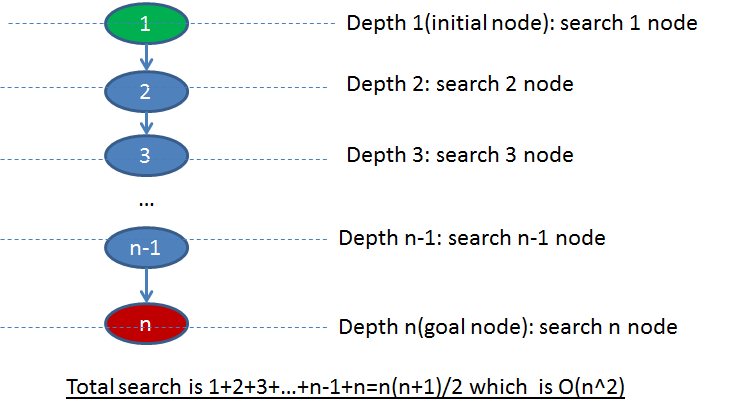
\includegraphics[width=0.8\columnwidth]{hw2_q2}\centering 
\caption{Illustrate the worst case for iterative deepen search}
\end{figure}


\item The text (page 95) describes consistency as:
\begin{eqnarray*}
h(n) &\leq c(n,a,n') + h(n')
\end{eqnarray*}
for state $n$, its successor $n'$ and action $a$.  For $G = (\{A,B,C\},\{(A,B), (A,C), (B,C)\})$, $Cost = \{((A,B),2), ((A,C),5), ((B,C), 1)\}$, and $h(A) = 1, h(B) = 4, h(C) = 3$. Is this consistent?\\
\underline{Answer to problem 3:} Yes, it is consistent, please see below figure for proof:
\begin{figure}[h]
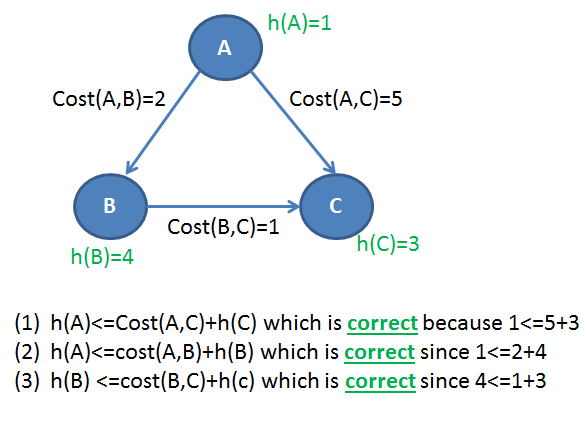
\includegraphics[width=0.8\columnwidth]{hw2_q3}\centering 
\caption{Illustrate the consistent heuristic function}
\end{figure}
  

\item Assume you're programming a robot named \textsf{R} to navigate a 2D surface.  The robot can only move forward a single step to an adjacent square (not diagonally), but can also rotate $\pm$ 90 degrees.  \textsf{R} has a single sensor on its front that determines if there is an obstruction, perhaps a wall, is in its path.  Your task is to read in a 2D plan and starting at location from the southmost (bottom) side, navigate to another side.  The plan below has an opening at (3,1).  {\it One} path is: (3,1), (3,2), $\ldots$, (3,5), (2,5), (1,5).  If \textsf{R} is at (4,2) facing north, then its sensor would return 1.  If \textsf{R} is at (4,2) and facing east, its sensor would return 0.  If \textsf{R} is at (2,2) facing west, to move to (3,2), rotate(90), rotate(90), step.  You can {\it start} \textsf{R} on any available open square on the bottom -- you'll have to decide what direction \textsf{R} is facing.  The plan is encoded as an array of ones and zeros.  The plan below:

\begin{center}
{\small
\begin{tikzpicture}
\draw[step=1cm,black,thin] (0,0) grid (6,6);
\draw[fill=blue](1,0) rectangle (2,1);
\draw[fill=blue](3,2) rectangle (4,3);
\draw[fill=blue](3,0) rectangle (4,1);
\draw[fill=blue](4,0) rectangle (5,1);
\draw[fill=blue](5,0) rectangle (6,1);
\draw[fill=blue](5,1) rectangle (6,2);
\draw[fill=blue](5,2) rectangle (6,3);
\draw[fill=blue](5,3) rectangle (6,4);
\draw[fill=blue](5,4) rectangle (6,5);
\draw[fill=blue](5,5) rectangle (6,6);
\draw[fill=blue](0,1) rectangle (1,2);
\draw[fill=blue](0,0) rectangle (1,1);
\draw[fill=blue](1,5) rectangle (2,6);
\draw[fill=blue](2,2) rectangle (3,3);
\draw[fill=blue](2,5) rectangle (3,6);
\draw[fill=blue](3,5) rectangle (4,6);
\draw[fill=blue](4,5) rectangle (5,6);
\draw[fill=blue](3,4) rectangle (4,5);
\draw[fill=blue](0,2) rectangle (1,3);
\draw[fill=blue](0,3) rectangle (1,4);
\draw[fill=blue](0,5) rectangle (1,6);
\draw[fill=blue](1,2) rectangle (2,3);
\end{tikzpicture}}
\end{center}

would be encoded as:

\begin{verbatim}
111111
000100
100001
111101
100001
110111
\end{verbatim}
\begin{enumerate}
\item Given a floor plan \texttt{f.txt} (read in the file),  return \textsf{True} and the series of instructions needed to navigate \textsf{R} if there is a path and \textsf{False} otherwise.  Name this program \texttt{rv1.py}.\\
\underline{Answer to question 4(a):}\\
Please check $hw2\_rv1.py$ for full code. I am using DFS search to get the path, and then using customized function $navigation\_path$ to print out the instructions as the following:
\begin{verbatim}
Here it is the shortest path by DFS search:
move to: (2, 0) facing to:  N
move to: (2, 1) facing to:  N
rotate+90
move to: (3, 1) facing to:  E
move to: (4, 1) facing to:  E
rotate-90
move to: (4, 2) facing to:  N
move to: (4, 3) facing to:  N
rotate-90
move to: (3, 3) facing to:  W
move to: (2, 3) facing to:  W
rotate+90
move to: (2, 4) facing to:  N
rotate-90
move to: (1, 4) facing to:  W
move to: (0, 4) facing to:  W
\end{verbatim}
\item Improve \textsf{R}'s programming by returning the {\it shortest} path if it exists.  Name this program \texttt{rv2.py}.\\
\underline{Answer to question 4(b):}\\
Using A start search(optimized by heuristic function) and print the navigation for robot. Please check the full code in $hw2\_rv2.py$.And here it is the running results:
\begin{verbatim}
Here it is the shortest path by A* search:
step to: (2, 0) facing to:  N
step to: (2, 1) facing to:  N
rotate+90
step to: (3, 1) facing to:  E
step to: (4, 1) facing to:  E
rotate-90
step to: (4, 2) facing to:  N
step to: (4, 3) facing to:  N
rotate-90
step to: (3, 3) facing to:  W
step to: (2, 3) facing to:  W
rotate+90
step to: (2, 4) facing to:  N
rotate-90
step to: (1, 4) facing to:  W
move to: (0, 4) facing to:  W
\end{verbatim}
\item Discuss your search techniques in both solutions.   State explicitly your $\hat{h}, \hat{g}, \hat{f}$.\\
\underline{Answer to question 4(c):}\\
My heuristic function is manhattan distance from the state to goal state. the actual cost is the movement cost: for 1 step is 10, for rotation, the actual cost is 0. the total cost is the actual cost plus heuristic cost.
so $\hat{f}=\hat{h}+\hat{g}$.\\
$\hat{h}=|x_0-x|+|y_0-y|$,   $(x_0,y_0)$ is goal cell coordination, $(x,y)$ is the current cell\\
$\hat{g_1}=\hat{g_0}+10$, $\hat{g_0}$ is previous actual cost, $\hat{g_1}$ is the actual cost after one step.\\
the rotation cost(+90 or -90) is zero.

\end{enumerate}
\item Extend Rock/Paper/Scissors from the last assignment that has the computer playing a human. You'll additionally have \$100 dollars worth of \$1 chips.  {\it Before} you show your selection, you must place a wager (at least \$1).  Keep the computer's strategy uniform and independent for both how it plays and how it bets.  The maximum amount of chips that can be wagered is $\mathrm{min}\{c,h\}$ where $c,h$ are the counts of computer and human chips respectively.  Compare this R/P/S with your earlier version and discuss.  Name this program \texttt{rpsg.py}. \\
\underline{Answer to question 5:}\\
\begin{itemize}
\item for each game round, Robby and computer will play 50 times or lose all chips(100 chips),then that round game over
\item Robby and computer played 50 the above game rounds
\item Robby and computer will show chips randomly
\item Robby will record the historic game records, he always show the opposite of the most common cards(R,P,S) which computer already  did.
\item The game results is exported to csv file(out.csv)
\item After analyzing game results, we found that Robby has 5039 chips, which is more than computers chips(4961).
\item By comparing chips for each round, Robby won 25 round games. But if compared with games quantity, Robby won 24 round games
\item Win games quantity does not mean winning chips.
\item the full code is in $hw2\_rpsg.py$, and the output csv file is in out.csv
\end{itemize}
\underline{Here it is another strategy:}
\begin{itemize}
\item Robby uses very conservative strategy to show chips: he only show 1 chip every round. 
\item Other strategy is the same as before. By using this strategy.
\item obby also win during the the test (I ran the program 2 times(every time 50 rimes 50 rounds game).
\item The output files are in out1.csv and out2.csv
\item Full code is in  $hw2\_rpsg\_v2.py$,
\end{itemize}
\end{enumerate}
\end{document}
